\documentclass[13pt,oneside]{book}
\usepackage[utf8]{inputenc}
\usepackage{url}
\usepackage{listings}
\usepackage{graphicx}

\usepackage{geometry}
\geometry{a4paper, left=20mm, right=20mm, top=20mm, bottom=20mm}
\usepackage[margin=1.2in]{geometry}
\usepackage[toc,page]{appendix}
\usepackage{graphicx}
\usepackage{natbib}
\usepackage{lipsum}
\usepackage{caption}

\begin{document}

\captionsetup[figure]{margin=1.5cm,font=small,labelfont={bf},name={Figure},labelsep=colon,textfont={it}}
\captionsetup[table]{margin=1.5cm,font=small,labelfont={bf},name={Table},labelsep=colon,textfont={it}}
\setlipsumdefault{1}

\begin{titlepage}
\begin{center}
{\LARGE College Of Engineering Trivandrum}\\[3cm]
\linespread{1.2}\huge {\bfseries System Software Lab}\\[3cm]
\linespread{1}

\includegraphics[width=5cm]{img/emblem.jpeg}\\[3cm]
{\Large GOKUL K\\ S5  CSE \\ Roll No:21\\ TVE18CS021 }\\[1cm]


\textit{ }\\[2cm]
Department of Computer Science\\[0.2cm]
\today
\end{center}

\end{titlepage}

\newpage

\begin{frame}{}
    \centering
    \hspace*{-0.5cm}
    $\vcenter{\hbox{
\includegraphics[width=1.5cm]{img/emblem.jpeg}}}$
    $\vcenter{\resizebox{0.95\textwidth}{!}{
        \begin{tabular}{c}
             CS331 - System Software Lab $\cdot$ 2020 $\cdot$   \\
             \hline 
        \end{tabular}
    }}$
\end{frame}
\section*{Cycle 2}
\section*{Expt 13}
\begin{center}
    \Large{Implementation of Relocating Loader}
\end{center}
\section*{Aim}
\large
To implement a relocating loader

\section*{Algorithm} 
    \begin{verbatim}
1 begin
2 read Header record
3 verify program name and length
4 read first Text record
5 Read the start address of relocation
6 Set addr to start
7 while record type != E do
8 begin
9 read bitmask convert it into binary
10 foreach opcode, address pair if the bit corresponding
  to it in bitmask is 1, relocate the address
11 print addr opcode relocated (or unrelocated) address
12 addr = addr + 3
13 end
14 jump to address specified in End record
15 end
	\end{verbatim}

\section*{Source Code}
\small

\begin{lstlisting}[language=C]
/* Implement a relocating loader */
#include <stdio.h>
#include <stdlib.h>
#include <string.h>

void convert(char[], char[]);

void main()
{
	FILE *objcode;
	int start_addr_in_mem, start_addr_in_prgrm;
	int prgrm_len, line_len, addr = 0, addr_in_mem, i = 0;
	char record_code, prgrm_name[10], prgrm_line[80];
	char *token, bitmask[30], binary_str[120], *opcode;

	if(! (objcode = fopen("objcode.txt", "r")))
	{
		printf("Please save the object code as objcode.txt\n");
		exit(0);
	}

	printf("Enter starting address in memory: ");
	scanf("%x", &start_addr_in_mem);

	while(! feof(objcode))
	{
		fscanf(objcode, "%c", &record_code);
		switch(record_code)
		{
			case 'H':
				fscanf(
					objcode, 
					"^%[^^]^%x^%x", 
					prgrm_name, 
					&start_addr_in_prgrm, 
					&prgrm_len
				);
				break;
			
			case 'T':
				fscanf(
					objcode, 
					"^%x^%x^%[^^]^%s", 
					&addr, 
					&line_len, 
					bitmask, prgrm_line
				);
				addr += start_addr_in_mem;
				convert(bitmask, binary_str);
				
				i = 0;

				// Splitting string with delimiter ^
				token = strtok(prgrm_line, "^");
				while(token != NULL)
				{
					addr_in_mem = (int) strtol(
						strtok(NULL, "^"),
						NULL,
						16
					);

					addr_in_mem = (binary_str[i++] == '0') 
						? addr_in_mem
						: addr_in_mem+start_addr_in_mem;
					printf("%x %s%x\n", addr, token, addr_in_mem);
					addr += 3;
					token = strtok(NULL, "^");
				}
				break;
			
			case 'E':
				exit(0);
		}
	}

	fclose(objcode);
}

void convert(char bitmask[], char binary_str[])
{
	int len = strlen(bitmask);
	strcpy(binary_str, "");
	
	for(int i = 0; i < len; i++)
	{
		switch(bitmask[i])
		{
			case '0':
				strcat(binary_str, "0000");
				break;
			case '1':
				strcat(binary_str, "0001");
				break;
			case '2':
				strcat(binary_str, "0010");
				break;
			case '3':
				strcat(binary_str, "0011");
				break;
			case '4':
				strcat(binary_str, "0100");
				break;
			case '5':
				strcat(binary_str, "0101");
				break;
			case '6':
				strcat(binary_str, "0110");
				break;
			case '7':
				strcat(binary_str, "0111");
				break;
			case '8':
				strcat(binary_str, "1000");
				break;
			case '9':
				strcat(binary_str, "1001");
				break;
			case 'A':
				strcat(binary_str, "1010");
				break;
			case 'B':
				strcat(binary_str, "1011");
				break;
			case 'C':
				strcat(binary_str, "1100");
				break;
			case 'D':
				strcat(binary_str, "1101");
				break;
			case 'E':
				strcat(binary_str, "1110");
				break;
			case 'F':
				strcat(binary_str, "1111");
				break;
		}
	}
} 
	
	\end{lstlisting}
	objcode.txt
	\begin{verbatim}
H^COPY^000000^00107A
T^000000^1E^FFC^14^0033^48^1039^10^0036^28^0030^30^0015^48^1061^3C^0003^20^002A^1C^0039^30^002D
T^002500^15^E00^1D^0036^48^1061^18^0033^4C^1000^80^1000^60^1003
E^000000		
	\end{verbatim}
	
    \section*{Output}
    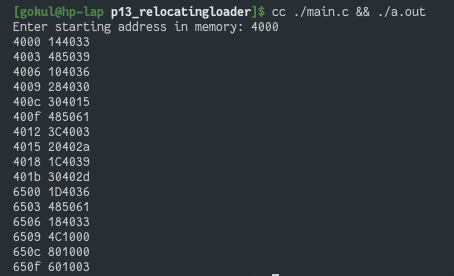
\includegraphics[width=\textwidth]{img/p13.png}
     
\Large
\section*{Result}
\large
Relocating loader is implemented and its output is verified
\end{document}